\documentclass[11pt]{article}

\usepackage{times}
\usepackage{epsf}
\usepackage{epsfig}
\usepackage{amsmath, alltt, amssymb, xspace}
\usepackage{wrapfig}
\usepackage{fancyhdr}
\usepackage{url}
\usepackage{verbatim}
\usepackage{fancyvrb}

\usepackage{subfigure}
\usepackage{cite}
%\usepackage{cases}
%\usepackage{ltexpprt}
%\usepackage{verbatim}

%\topmargin      -0.70in  % distance to headers
%\headheight     0.2in   % height of header box
%\headsep        0.4in   % distance to top line
%\footskip       0.3in   % distance from bottom line

% Horizontal alignment
\topmargin      -0.50in  % distance to headers
\oddsidemargin  0.0in
\evensidemargin 0.0in
\textwidth      6.5in
\textheight     8.9in 


%\centerfigcaptionstrue

%\def\baselinestretch{0.95}


\newcommand\discuss[1]{\{\textbf{Discuss:} \textit{#1}\}}
%\newcommand\todo[1]{\vspace{0.1in}\{\textbf{Todo:} \textit{#1}\}\vspace{0.1in}}
\newtheorem{problem}{Problem}[section]
%\newtheorem{theorem}{Theorem}
%\newtheorem{fact}{Fact}
\newtheorem{define}{Definition}[section]
%\newtheorem{analysis}{Analysis}
\newcommand\vspacenoindent{\vspace{0.1in} \noindent}

%\newenvironment{proof}{\noindent {\bf Proof}.}{\hspace*{\fill}~\mbox{\rule[0pt]{1.3ex}{1.3ex}}}
%\newcommand\todo[1]{\vspace{0.1in}\{\textbf{Todo:} \textit{#1}\}\vspace{0.1in}}

%\newcommand\reducespace{\vspace{-0.1in}}
% reduce the space between lines
%\def\baselinestretch{0.95}

\newcommand{\fixmefn}[1]{ \footnote{\sf\ \ \fbox{FIXME} #1} }
\newcommand{\todo}[1]{
\vspace{0.1in}
\fbox{\parbox{6in}{TODO: #1}}
\vspace{0.1in}
}

\newcommand{\mybox}[1]{
\vspace{0.2in}
\noindent
\fbox{\parbox{6.5in}{#1}}
\vspace{0.1in}
}


\newcounter{question}
\setcounter{question}{1}

\newcommand{\myquestion} {{\vspace{0.1in} \noindent \bf Question \arabic{question}:} \addtocounter{question}{1} \,}

\newcommand{\myproblem} {{\noindent \bf Problem \arabic{question}:} \addtocounter{question}{1} \,}


\newcommand{\copyrightnoticeA}[1]{
\vspace{0.1in}
\fbox{\parbox{6in}{\small Copyright \copyright\ 2006 - 2014\ \ Wenliang Du, Syracuse University.\\ 
      The development of this document is partially funded by 
      the National Science Foundation's Course, Curriculum, and Laboratory 
      Improvement (CCLI) program under Award No. 0618680 and 0231122. 
      Permission is granted to copy, distribute and/or modify this document
      under the terms of the GNU Free Documentation License, Version 1.2
      or any later version published by the Free Software Foundation.
      A copy of the license can be found at http://www.gnu.org/licenses/fdl.html.}}
\vspace{0.1in}
}


\newcommand{\copyrightnotice}[1]{
\vspace{0.1in}
\fbox{\parbox{6in}{\small Copyright \copyright\ 2006 - 2014\ \ Wenliang Du, Syracuse University.\\
      The development of this document is/was funded by three grants from
      the US National Science Foundation: Awards No. 0231122 and 0618680 from
      TUES/CCLI and  Award No. 1017771 from Trustworthy Computing.
      This lab was imported into the Labtainer framework by the Naval Postgraduate 
      School, Center for Cybersecurity and Cyber Operations under National Science 
      Foundation Award No. 1438893.
      Permission is granted to copy, distribute and/or modify this document
      under the terms of the GNU Free Documentation License, Version 1.2
      or any later version published by the Free Software Foundation.
      A copy of the license can be found at http://www.gnu.org/licenses/fdl.html.}}
\vspace{0.1in}
}

\newcommand{\copyrightnoticeB}[1]{
\vspace{0.1in}
\fbox{\parbox{6in}{\small Copyright \copyright\ 2006 - 2014\ \ Wenliang Du, Syracuse University.\\
      The development of this document is/was funded by the following grants from
      the US National Science Foundation: No. 0231122, 0618680, and 1303306.
      Permission is granted to copy, distribute and/or modify this document
      under the terms of the GNU Free Documentation License, Version 1.2
      or any later version published by the Free Software Foundation.
      A copy of the license can be found at http://www.gnu.org/licenses/fdl.html.}}
\vspace{0.1in}
}


\newcommand{\nocopyrightnotice}[1]{
\vspace{0.1in}
\fbox{\parbox{6in}{\small  
      The development of this document is funded by 
      the National Science Foundation's Course, Curriculum, and Laboratory 
      Improvement (CCLI) program under Award No. 0618680 and 0231122. 
      Permission is granted to copy, distribute and/or modify this document.
      }}
\vspace{0.1in}
}

\newcommand{\idea}[1]{
\vspace{0.1in}
{\sf IDEA:\ \ \fbox{\parbox{5in}{#1}}}
\vspace{0.1in}
}

\newcommand{\questionblock}[1]{
\vspace{0.1in}
\fbox{\parbox{6in}{#1}}
\vspace{0.1in}
}


\newcommand{\minix}{{\tt Minix}\xspace}
\newcommand{\unix}{{\tt Unix}\xspace}
\newcommand{\linux}{{\tt Linux}\xspace}
\newcommand{\ubuntu}{{\tt Ubuntu}\xspace}
\newcommand{\selinux}{{\tt SELinux}\xspace}
\newcommand{\freebsd}{{\tt FreeBSD}\xspace}
\newcommand{\solaris}{{\tt Solaris}\xspace}
\newcommand{\windowsnt}{{\tt Windows NT}\xspace}
\newcommand{\setuid}{{\tt Set-UID}\xspace}
%\newcommand{\smx}{{\tt Smx}\xspace}
\newcommand{\smx}{{\tt Minix}\xspace}
\newcommand{\relay}{{\tt relay}\xspace}
\newcommand{\isys}{{\tt iSYS}\xspace}
\newcommand{\ilan}{{\tt iLAN}\xspace}
\newcommand{\iSYS}{{\tt iSYS}\xspace}
\newcommand{\iLAN}{{\tt iLAN}\xspace}
\newcommand{\iLANs}{{\tt iLAN}s\xspace}
\newcommand{\bochs}{{\tt Bochs}\xspace}

\newcommand\FF{{\mathcal{F}}}

\newcommand{\argmax}[1]{
\begin{minipage}[t]{1.25cm}\parskip-1ex\begin{center}
argmax
#1
\end{center}\end{minipage}
\;
}

\newcommand{\bm}{\boldmath}
\newcommand  {\bx}    {\mbox{\boldmath $x$}}
\newcommand  {\by}    {\mbox{\boldmath $y$}}
\newcommand  {\br}    {\mbox{\boldmath $r$}}


%\pagestyle{fancyplain}
%\lhead[\thepage]{\thesection}      % Note the different brackets!
%\rhead[\thesection]{SEED Laboratories}
%\lfoot[\fancyplain{}{}]{Syracuse University} 
%\cfoot[\fancyplain{}{}]{\thepage} 

\newcommand{\tstamp}{\today}   
%\lhead[\fancyplain{}{\thepage}]         {\fancyplain{}{\rightmark}}
%\chead[\fancyplain{}{}]                 {\fancyplain{}{}}
%\rhead[\fancyplain{}{\rightmark}]       {\fancyplain{}{\thepage}}
%\lfoot[\fancyplain{}{}]                 {\fancyplain{\tstamp}{\tstamp}}
%\cfoot[\fancyplain{\thepage}{}]         {\fancyplain{\thepage}{}}
%\rfoot[\fancyplain{\tstamp} {\tstamp}]  {\fancyplain{}{}}

\pagestyle{fancy}
%\lhead{\bfseries Computer Security Course Project}
\lhead{\bfseries SEED Labs}
\chead{}
\rhead{\small \thepage}
\lfoot{}
\cfoot{}
\rfoot{}

\usepackage{listings}
\usepackage{color}

\definecolor{dkgreen}{rgb}{0,0.6,0}
\definecolor{gray}{rgb}{0.5,0.5,0.5}
\definecolor{mauve}{rgb}{0.58,0,0.82}

\lstset{frame=tb,
  language=C,
  aboveskip=3mm,
  belowskip=3mm,
  showstringspaces=false,
  columns=flexible,
  basicstyle={\small\ttfamily},
  numbers=none,
  numberstyle=\tiny\color{gray},
  keywordstyle=\color{blue},
  commentstyle=\color{dkgreen},
  stringstyle=\color{mauve},
  breaklines=true,
  breakatwhitespace=true,
  tabsize=3
}




%\documentclass{article} 
%\usepackage{graphicx}
%\usepackage{color}
%\usepackage[latin1]{inputenc}
%\usepackage{lgrind}
%\input {highlight.sty}

\lhead{\bfseries SEED Labs -- Return-to-libc Attack Lab}


\def \code#1 {\fbox{\scriptsize{\texttt{#1}}}}

\begin{document}

\begin{center}
{\LARGE Return-to-libc Attack Lab}
\end{center}

\copyrightnotice

\section{Lab Overview}
The learning objective of this lab is for students to gain 
first-hand experience with a variant of the buffer-overflow
attack; this attack can bypass a protection scheme currently
implemented in major Linux operating systems.  A common way to exploit
a buffer-overflow vulnerability is to overflow the buffer with 
malicious shellcode, and then cause the vulnerable program to jump to
the shellcode that is stored in the stack. To prevent these types of
attacks, some operating systems provide an ability
to make stacks non-executable; therefore, jumping to
the shellcode will cause the program to fail.

Unfortunately, the above protection scheme is not fool-proof; there
exists a variant of buffer-overflow attack called the {\tt
  return-to-libc} attack, which does not need an executable stack; it
does not even use shell code. Instead, it causes the vulnerable
program to jump to some existing code, such as the {\tt system()}
function in the {\tt libc} library, which is already loaded into the
memory.

In this lab, students are given a program with a buffer-overflow
vulnerability; their task is to develop a {\tt return-to-libc} attack
to exploit the vulnerability and finally to gain the root privilege.
In addition to the attacks, students will be guided to walk through
several protection schemes that have been implemented in Ubuntu to
counter against the buffer-overflow attacks. Students need to evaluate
whether the schemes work or not and explain why.
\section{Lab Environment}
This lab runs in the Labtainer framework,
available at http://my.nps.edu/web/c3o/labtainers.
That site includes links to a pre-built virtual machine
that has Labtainers installed, however Labtainers can
be run on any Linux host that supports Docker containers.

From your labtainer-student directory start the lab using:
\begin{verbatim}
    labtainer retlibc
\end{verbatim}
Links to this lab manual and to an empty lab report will be displayed.  If you create your lab report on a separate system,
be sure to copy it back to the specified location on your Linux system.


\section{Lab Tasks}
You are required to exploit the "retlib" program.  You are provided the
source code to the program, but you are not to alter the program source code.

\subsection{Initial Setup}

\paragraph{Address Space Randomization.}
\ubuntu and several other Linux-based systems uses address space
randomization to randomize the starting address of heap and
stack. This makes guessing the exact addresses difficult; guessing
addresses is one of the critical steps of buffer-overflow attacks.  In
this lab, we disable this feature using the following command:

\begin{verbatim}
  sudo sysctl -w kernel.randomize_va_space=0
\end{verbatim}


\paragraph{The StackGuard Protection Scheme.}
The GCC compiler implements a security mechanism called
"Stack Guard" to prevent buffer overflows. In the presence of this
protection, buffer overflows will fail. You can disable this
protection if you compile the program using the
\emph{-fno-stack-protector} switch. For example, to compile a program
example.c with Stack Guard disabled, you may use the following command:
\begin{verbatim}
  $ gcc -m32 -fno-stack-protector example.c
\end{verbatim}

The retlib program was compiled without StackGuard.

\paragraph{Non-Executable Stack.} \ubuntu used to allow executable stacks,
but this has now changed: the binary images of programs (and shared
libraries) must declare whether they require executable stacks or not,
i.e., they need to mark a field in the program header. The kernel or dynamic
linker uses this marking to decide whether to make the stack of this
running program executable or non-executable. This marking is done
automatically by the recent versions of {\tt gcc}, and by default, the
stack is set to be non-executable.  
To change that, use the following option when compiling programs:
\begin{verbatim}
  For executable stack:
  $ gcc -m32 -z execstack  -o test test.c

  For non-executable stack:
  $ gcc -m32 -z noexecstack  -o test test.c
\end{verbatim}


Because the objective of this lab is to show that the non-executable stack
protection does not work, the retlib program was compiled with the 
{\tt "-z noexecstack"} option.


\paragraph {Note for Instructors:} 
For this lab, a lab session is desirable, especially if students are
not familiar with the tools and the enviornments. If an instructor
plans to hold a lab session (by himself/herself or by a TA), it
is suggested the following to be covered in the
lab session~\footnote{We assume that the instructor has already covered
the concepts of the attacks in the lecture, so we do not include
them in the lab session.}:
\begin{enumerate}
  \item The use of Labtainers. 

  \item Basic use of {\tt gdb} debug commands and stack stucture.

\end{enumerate}

Review the retlib.c program.
It has a buffer overflow vulnerability. It first reads
an input of size 80 bytes from a file called ``badfile'' into a buffer
that is smaller than 80 bytes, causing the overflow. The function fread() does not check
boundaries, so a buffer overflow will occur.  Since this program is a
set-root-uid program, if a normal user can exploit this buffer
overflow vulnerability, the normal user might be able to get a root
shell.  It should be noted that the program gets its input from a file
called ``badfile''. This file is under the users' control. Our
objective is to create the contents for ``badfile'', such that when
the vulnerable program copies the contents into its buffer, a root
shell can be spawned.

\subsection{Task 1: Exploiting the Vulnerability} 
Create the \textbf{badfile}. Your home directory includes an "exploit.c" program
that you can modify in order to create the badfile.

You need to figure out the values for the addresses in that program, as well 
as where to store those addresses. If you incorrectly calculate
the locations, your attack might not work.

After you modify the exploit.c program, compile using \texttt{compile\_exploit.sh} 
and run it; this will
generate the contents for ``badfile''. Run the vulnerable program {\tt
  retlib}. If your exploit is implemented correctly, when the function
{\tt bof} returns, it will return to the {\tt system()} libc function,
and execute {\tt system("/bin/sh")}. If the vulnerable program is
running with the root privilege, you can get the root shell at this
point.

It should be noted that the {\tt exit()} function is not very
necessary for this attack; however, without this function, when {\tt
  system()} returns, the program might crash, causing suspicions.

\begin{verbatim}
  $ ./compile_exploit.sh
  $./exploit         // create the badfile
  $./retlib          // launch the attack by running the vulnerable program
  # <---- You've got a root shell! 
\end{verbatim}


\paragraph{Questions.} In your report, please answer the following questions:
\begin{itemize}
\item Please describe how you decide the values for {\tt X}, {\tt Y} and {\tt
Z}. Either show us your reasoning, or if you use trial-and-error approach,
show your trials.

\item After your attack is successful, change the file name of {\tt retlib}
to a different name, making sure that the length of the file names are
different. For example, you can change it to {\tt newretlib}. Repeat the
attack (without changing the content of {\tt badfile}). Is your attack
successful or not? If it does not succeed, explain why.

\end{itemize}


\subsection{Task 2: Address Randomization}

In this task, let us turn on the Ubuntu's address randomization protection.  
We run the same attack developed in Task 1. Can you get a shell? If not, 
what is the problem? How does the address randomization
make your return-to-libc attack difficult?
You should describe your observation and explanation
in your lab report. You can use the following instructions to turn
on the address randomization:

\begin{verbatim}
  sudo sysctl -w kernel.randomize_va_space=2
\end{verbatim}



\subsection{Task 3: Stack Guard Protection}

In this task, let us turn on the Ubuntu's Stack Guard protection.  
Please remember to turn off the address randomization protection. 
We run the same attack developed in Task 1. Can you get a shell? If not, 
what is the problem? How does the Stack Guard protection
make your return-to-libc attack difficult?
You should describe your observation and explanation
in your lab report. You can use the following instructions to compile
your program with the Stack Guard protection turned on.

\begin{verbatim}
  sudo su
  # gcc -m32 -z noexecstack  -o retlib retlib.c
  # chmod 4755 retlib
  # exit  
\end{verbatim}


\section{Guidelines: Understanding the function call mechanism}

\subsection{Find out the addresses of libc functions} 

To find out the address of any libc function, you can use the following
{\tt gdb} commands ({\tt a.out} is an arbitrary program):
\begin{verbatim}
 $ gdb a.out

 (gdb) b main
 (gdb) r
 (gdb) p system
  $1 = {<text variable, no debug info>} 0x9b4550 <system>
 (gdb) p exit
  $2 = {<text variable, no debug info>} 0x9a9b70 <exit>
\end{verbatim}

From the above {\tt gdb} commands, we can find out that the address 
for the {\tt system()} function is {\tt 0x9b4550}, and the address
for the {\tt exit()} function is {\tt 0x9a9b70}. The actual addresses
in your system might be different from these numbers.


\subsection{Putting the shell string in the memory}

One of the challenge in this lab is to put the string {\tt "/bin/sh"}
into the memory, and get its address. This can be achieved using 
environment variables.
When a C program is executed, it inherits all the environment variables from
the shell that executes it. The environment variable \textbf{SHELL} points
directly to \texttt{/bin/bash} and is needed by other programs, so we introduce
a new shell variable \textbf{MYSHELL} and make it point to \texttt{zsh} \\

\begin{verbatim}
  $ export MYSHELL=/bin/sh
\end{verbatim}

We will use the address of this variable as an argument to {\tt system()} call.
The location of this variable in the memory can be found out easily using the 
following program: 
\begin{verbatim}
  void main(){
    char* shell =  getenv("MYSHELL");
    if (shell) 
       printf("%x\n", (unsigned int)shell);
  }
\end{verbatim}

If the address randomization is turned off, you will find out that the same 
address is printed out. However, when you run the 
vulnerabile program {\tt retlib}, the address of the environment
variable might not be exactly the same as the one that you get by running 
the above program; such an address can even change when you change
the name of your program (the number of characters in the file
name makes difference). The good news is, the address of the shell will
be quite close to what you print out using the above program. Therefore,
you might need to try a few times to succeed.


\subsection{Understand the Stack}

To know how to conduct the {\tt return-to-libc} attack, it is essential to 
understand how the stack works.  We use a small C program to understand 
the effects of a function invocation on the stack. 
\begin{verbatim}
/* foobar.c */
#include<stdio.h>
void foo(int x)
{
  printf("Hello world: %d\n", x);
}

int main()
{
  foo(1);
  return 0;
}
\end{verbatim}
We can use {\tt "gcc -m32 -S foobar.c"} to
compile this program to the assembly code.
The resulting file {\tt foobar.s} will look like the following:
\begin{verbatim}
    ......
  8 foo:
  9         pushl   %ebp
 10         movl    %esp, %ebp
 11         subl    $8, %esp
 12         movl    8(%ebp), %eax   
 13         movl    %eax, 4(%esp)
 14         movl    $.LC0, (%esp)  : string "Hello world: %d\n"
 15         call    printf
 16         leave
 17         ret
    ......
 21 main:
 22         leal    4(%esp), %ecx
 23         andl    $-16, %esp
 24         pushl   -4(%ecx)
 25         pushl   %ebp
 26         movl    %esp, %ebp
 27         pushl   %ecx
 28         subl    $4, %esp
 29         movl    $1, (%esp)
 30         call    foo
 31         movl    $0, %eax
 32         addl    $4, %esp
 33         popl    %ecx
 34         popl    %ebp
 35         leal    -4(%ecx), %esp
 36         ret
\end{verbatim}

\subsection{Calling and Entering {\tt foo()}}

Let us concentrate on the stack while calling {\tt foo()}. We can ignore the stack
before that. Please note that line numbers instead of instruction addresses are
used in this explanation. 

\begin{figure}[t]
   \begin{center} 
   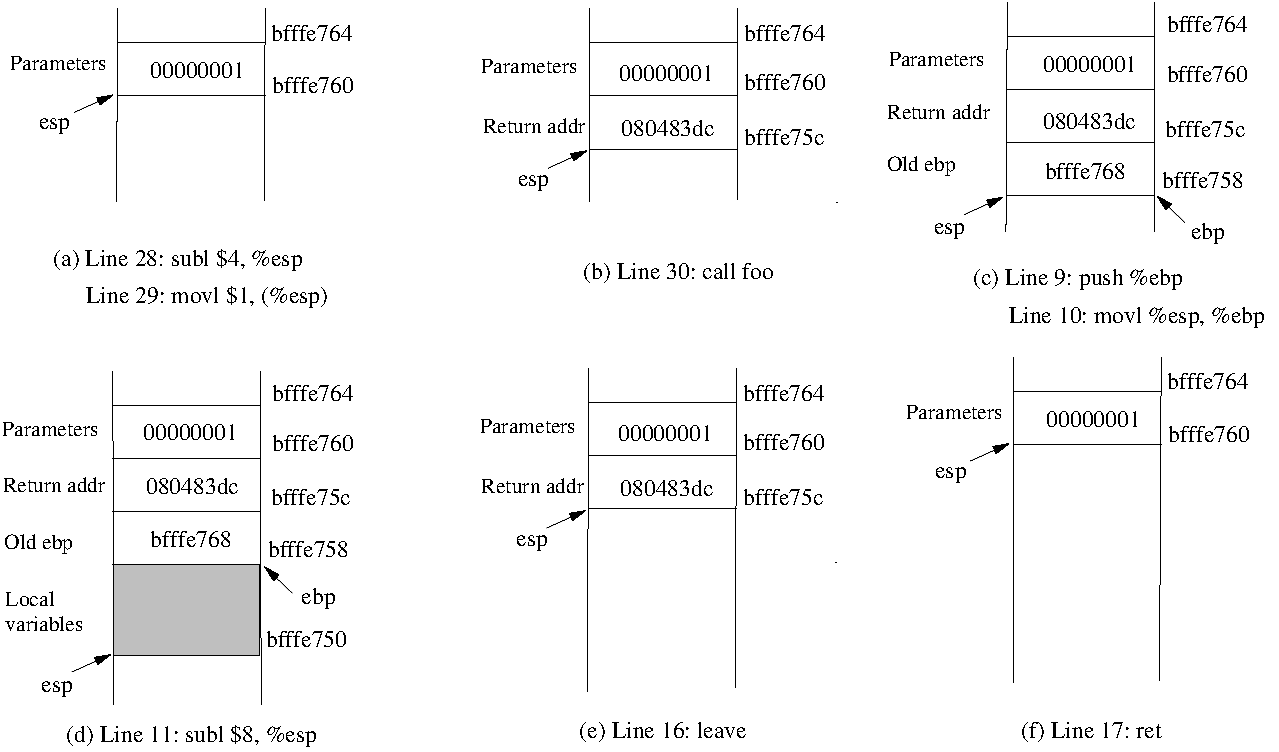
\includegraphics[width=0.9\textwidth,natwidth=621,natheight=403]{Figs/enter_leave_foo.pdf}
    \end{center}
    \caption{Entering and Leaving {\tt foo()}}
    \label{fig:enter_leave_foo}
\end{figure}



\begin{itemize}
\item \textbf{Line 28-29:}:
These two statements push the value $1$, i.e. the argument to the {\tt foo()}, 
into the stack. This operation increments {\tt \%esp} by four. The stack
after these two statements is depicted in Figure~\ref{fig:enter_leave_foo}(a).

\item \textbf{Line 30: \texttt{call foo}}: 
The statement pushes the address of the next instruction that 
immediately follows the {\tt call} statement into the 
stack (i.e the return address), and then jumps to the 
code of {\tt foo()}. 
The current stack is depicted in Figure~\ref{fig:enter_leave_foo}(b).

\item \textbf{Line 9-10}:
The first line of the function {\tt foo()} pushes {\tt \%ebp} into
the stack, to save the previous frame pointer. The second
line lets {\tt \%ebp} point to the current frame. The current stack 
is depicted in Figure~\ref{fig:enter_leave_foo}(c). 

\item \textbf{Line 11: \texttt{subl \$8, \%esp}}:
The stack pointer is modified to allocate space (8 bytes) for 
local variables and the two arguments passed to {\tt printf}. 
Since there is no local variable in function {\tt foo}, the
8 bytes are for arguments only. 
See Figure~\ref{fig:enter_leave_foo}(d). 

\end{itemize}


\subsection{Leaving {\tt foo()}}

Now the control has passed to the function {\tt foo()}. Let us see what happens
to the stack when the function returns.

\begin{itemize}
\item \textbf{Line 16: \texttt{leave}}: This
instruction implicitly performs two instructions (it was a macro
in earlier x86 releases, but was made into an instruction later):
\begin{verbatim}
    mov  %ebp, %esp
    pop  %ebp
\end{verbatim}
The first statement release the stack space allocated for the function; 
the second statement recover the previous frame pointer. 
The current stack is depicted in Figure~\ref{fig:enter_leave_foo}(e). 

\item \textbf{Line 17: \texttt{ret}}: This instruction simply pops the return 
address out of the stack, and then jump to the return address.
The current stack is depicted in Figure~\ref{fig:enter_leave_foo}(f).

\item \textbf{Line 32: \texttt{addl \$4, \%esp}}: Further resotre the stack by
releasing more memories allocated for {\tt foo}. 
As you can clearly see that the stack is now in exactly the same state as it was
before entering the function {\tt foo} (i.e., before line 28). 
\end{itemize}


%\subsection{Brief description of system() call}
%The function call mechanism described above differs slightly from the system call mechanism. The exact procedure varies with the libc library, the kernel version and even the distribution you are using. The call mechanism on Fedora Core 4(and 5) using libc version 2.3.5 is explained here (You can find the libc version by typing \texttt{/lib/libc.so.6} at the prompt). 

%The system() function is not called directly, the lookup functions are called first, but for the purpose of simplicity, we will ignore those details and jump right into system() code:
%\begin{verbatim}
%/* source/sysdeps/posix/system.c */
%int
%__libc_system (const char *line)
%{
%  if (line == NULL)
%    return do_system ("exit 0") == 0;
%
%  if (SINGLE_THREAD_P)
%    return do_system (line);
%
%  int oldtype = LIBC_CANCEL_ASYNC ();
%
%  int result = do_system (line);
%
%  LIBC_CANCEL_RESET (oldtype);
%
%  return result;
%}
%weak_alias (__libc_system, system)
%
%\end{verbatim}
%We can see that system() is an alias of \texttt{\_\_libc\_system}. The macro \texttt{weak\_alias} takes care of lower level type checking and other functionalities provided by GCC's \texttt{\_\_attribute\_\_} method. We can see that the function \texttt{do\_system()} does most of system's work. It will be sufficient to see whether the location of data before the call to do\_system() still satisfies the assumptions necessary for the success of our attack. . Lets see the assembly code for system:
%\begin{verbatim}
%0x0032a3df <system+0>:  push   %edi
%0x0032a3e0 <system+1>:  push   %esi
%0x0032a3e1 <system+2>:  push   %ebx
%0x0032a3e2 <system+3>:  call   0x309c60 <__i686.get_pc_thunk.bx>
%0x0032a3e7 <system+8>:  add    $0xf0c0d,%ebx
%0x0032a3ed <system+14>: mov    0x10(%esp),%edi
%0x0032a3f1 <system+18>: test   %edi,%edi
%0x0032a3f3 <system+20>: je     0x32a409 <system+42>
%0x0032a3f5 <system+22>: mov    %gs:0xc,%eax
%0x0032a3fb <system+28>: test   %eax,%eax
%0x0032a3fd <system+30>: jne    0x32a422 <system+67>
%0x0032a3ff <system+32>: mov    %edi,%eax
%0x0032a401 <system+34>: pop    %ebx
%0x0032a402 <system+35>: pop    %esi
%0x0032a403 <system+36>: pop    %edi
%0x0032a404 <system+37>: jmp    0x329f3c <do_system>
%
%\end{verbatim}
%Consider the following sample program used for testing purposes:
%\begin{verbatim}
%#include<stdio.h>
%void mysys(char *x)
%{
%   char c[5];
%   system("/bin/sh");
%   c[2]='s';
%}
%int main()
%{
%   mysys("hello");
%}
%\end{verbatim}
%
%Let us inspect the data, before jumping to \texttt{do\_system()}, in the assembly
%code of system. The following GDB log entries might be helpful:
%
%\begin{verbatim}
% 	1 0x0032a404 in system () from /lib/libc.so.6
%  2 (gdb) x $esp+4
%  3 0xbffff800:     0x0804846c
%  4 (gdb) x/s 0x0804846c
%  5 0x804846c <_IO_stdin_used+4>:    "/bin/sh"
%  6 (gdb) x/x $ebp+4
%  7 0xbffff82c:     0x080483c1
%  8 (gdb) disassemble main
%  9 Dump of assembler code for function main:
% 10 0x08048398 <main+0>:    push   %ebp
% 11 0x08048399 <main+1>:    mov    %esp,%ebp
% 12 0x0804839b <main+3>:    sub    $0x8,%esp
% 13 0x0804839e <main+6>:    and    $0xfffffff0,%esp
% 14 0x080483a1 <main+9>:    mov    $0x0,%eax
% 15 0x080483a6 <main+14>:   add    $0xf,%eax
% 16 0x080483a9 <main+17>:   add    $0xf,%eax
% 17 0x080483ac <main+20>:   shr    $0x4,%eax
% 18 0x080483af <main+23>:   shl    $0x4,%eax
% 19 0x080483b2 <main+26>:   sub    %eax,%esp
% 20 0x080483b4 <main+28>:   sub    $0xc,%esp
% 21 0x080483b7 <main+31>:   push   $0x8048474
% 22 0x080483bc <main+36>:   call   0x804837c <mysys>
% 23 0x080483c1 <main+41>:   add    $0x10,%esp
% 24 0x080483c4 <main+44>:   leave
% 25 0x080483c5 <main+45>:   ret
% 26 End of assembler dump.
%\end{verbatim}

%Looking at the disassembly of the main function we can quite clearly see that the return address for the function \texttt{mysys()} is \texttt{0x08048c1}. We know that the this return address is stored in address next to the frame pointer, which is stored in EBP. Line 6 above shows that this indeed is the case, but why isn't the frame pointer changed? The reason is that; on FC4 and 5, the system() call spawns a new process, and execs the shell along with the parameter supplied to it. So since that process is a mirror image of the original program, it retains the old registers and frame pointers. 
%
%Line 2 through 5 shows the presence of the string "/bin/sh" on the stack. Hence we quite clearly see that structure of the attack should not change when attacking the library calls. The stack may be displaced but the structure is essentially similar.


\begin{thebibliography}{10}

\bibitem{c0ntext}
c0ntext
\newblock Bypassing non-executable-stack during exploitation using return-to-libc
\newblock http://www.infosecwriters.com/text\_resources/pdf/return-to-libc.pdf 

\bibitem{Phrack}
Phrack by Nergal
\newblock Advanced return-to-libc exploit(s) 
\newblock {\em Phrack 49}, Volume 0xb, Issue 0x3a. Available at
				http://www.phrack.org/archives/58/p58-0x04
\end{thebibliography}
\end{document}
